% --- IMPORTS ---
\documentclass[leqno]{article}
\usepackage{graphicx}
\usepackage{dsfont}
\usepackage{mathtools}
\usepackage{amssymb}
\usepackage{amsmath}
\usepackage{amsthm}
\usepackage{float}
\usepackage{ragged2e}
\usepackage{tensor}
\usepackage{fancyhdr}
\usepackage{empheq}
\usepackage[most]{tcolorbox}
\usepackage{enumitem}
\usepackage{dirtytalk}
\usepackage{marginnote}
\usepackage{microtype}
\usepackage[
  a4paper,
  left=0.8in,
  right=1in,
  top=1in,
  bottom=0.5in,
  headheight=14pt,
  headsep=0.4in
]{geometry}
\setlength{\parindent}{0cm}
% --- TikZ Packages ---
\usepackage{pgfplots}
\pgfplotsset{compat=1.18}
\usepgfplotslibrary{fillbetween, polar}
\usetikzlibrary{calc, positioning}
\usetikzlibrary{angles, quotes}
\usetikzlibrary{arrows.meta}
\usetikzlibrary{decorations.pathreplacing, decorations.markings}
\usetikzlibrary{patterns}
\usetikzlibrary{intersections}
% --- URL Packages ---
\usepackage[colorlinks=true,linkcolor=red,citecolor=magenta,urlcolor=black]{hyperref}%
\urlstyle{same}
% --- END OF IMPORTS ---

% --- CUSTOM COMMANDS ---
\RenewDocumentCommand{\marks}{o m}{%
  \IfValueTF{#1}%
    {\marginnote{\raggedright\textbf{[#2]}}[#1]}%
    {\marginnote{\raggedright\textbf{[#2]}}}%
}
\newcommand{\vspacerule}[2]{%
  \par\vspace*{#1}%
  \noindent\hrulefill\par
  \vspace*{#2}%
}
\definecolor{scarlet}{RGB}{205, 40, 75}
\newcommand{\questionitem}{%
  \item\phantomsection
  \addcontentsline{toc}{section}{Question \number\value{enumi}}%
}
\renewcommand{\contentsname}{Questions}
\newcommand{\timingbox}[4]{%
  \vspace*{20pt}
  \noindent\begin{tcolorbox}[
    enhanced, sharp corners,
    width=0.8\textwidth,
    colback=white, colframe=white, boxrule=0pt,
    borderline west={3pt}{0pt}{scarlet},
    left=20pt, right=20pt, top=12pt, bottom=12pt,
    before skip=0pt, after skip=0pt
  ]
  {\LARGE\bfseries #1}\\[8pt]
  {\normalsize Total Marks: #2 }\\[6pt]
  {\normalsize  #3\\[6pt]
  Complete in \textbf{#4}}
  \end{tcolorbox}
  \vspace*{20pt}%
}
% --- END OF CUSTOM COMMANDS ---

% --- HEADER CONFIG ---
\pagestyle{fancy}
\fancyhead{}
\fancyfoot{}
\renewcommand{\headrulewidth}{0.9pt}
\lhead{Collisions in 2 Dimensions}
\chead{}
\rhead{\href{https://danieljsmith.org}{danieljsmith.org}}
% --- END OF HEADER CONFIG ---

\begin{document}
\vspace*{20pt}
\tableofcontents
\newpage
\begin{enumerate}[
  label=\textbf{\arabic*.},
  leftmargin=*,
  topsep=0pt,
  partopsep=0pt,
  parsep=0pt
]

% ---- Question 1 ----
\questionitem
% [Source: _QBT__Collisions_in_2_Dimensions, Q1]

\begin{figure}[H]
    \centering
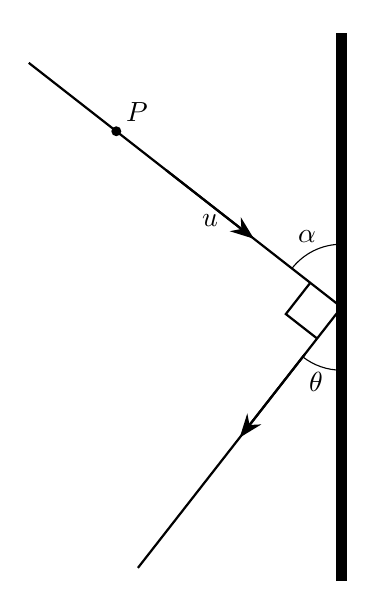
\begin{tikzpicture}[scale=1.2]
\def\alphaang{52}
\def\thetaang{38}
\def\inclen{4.2}
\def\outlen{3.5}
\def\wallht{2.9}
\def\marklen{0.42}

\coordinate (C) at (0,0);
\coordinate (U) at (0,1.5);
\coordinate (D) at (0,-1.5);
\coordinate (I) at ({90+\alphaang}:\inclen);
\coordinate (R) at ({270-\thetaang}:\outlen);
\coordinate (P) at ($(C)!0.72!(I)$);
\coordinate (uA) at ($(C)!0.28!(I)$);
\coordinate (uB) at ($(C)!0.56!(I)$);
\coordinate (vA) at ($(C)!0.18!(R)$);
\coordinate (vB) at ($(C)!0.50!(R)$);
\coordinate (Q1) at ({90+\alphaang}:\marklen);
\coordinate (Q2) at ({270-\thetaang}:\marklen);
\coordinate (Q3) at ($(Q1)+(Q2)-(C)$);

\draw[line width=4pt] (0,-\wallht) -- (0,\wallht);
\draw[thick] (I) -- (C) -- (R);

\draw[-{Stealth[length=3mm]}, thick] (uB) -- (uA) node[midway, below] {$u$};
\draw[-{Stealth[length=3mm]}, thick] (vA) -- (vB);

\draw[thick] (Q1) -- (Q3) -- (Q2);

\fill (P) circle (1.5pt);
\node[above right] at (P) {$P$};

\pic["$\alpha$", draw, angle radius=8mm, angle eccentricity=1.25] {angle=U--C--I};
\pic["$\theta$", draw, angle radius=8mm, angle eccentricity=1.25] {angle=R--C--D};
\end{tikzpicture}
\end{figure}


A particle $P$ of mass $m$ is moving with speed $u$ on a fixed smooth horizontal surface. It collides with a fixed smooth vertical barrier. Before impact its path makes an angle $\alpha$ with the barrier, and after impact its path makes an angle $\theta$ with the barrier. The incident path and the outgoing path are perpendicular. The coefficient of restitution between $P$ and the barrier is $e$. The particle loses $36\%$ of its kinetic energy in the collision. \\

Find the value of $e$ and the exact value of $\tan \alpha$. \marks{5}

\newpage


% ---- Question 2 ----
\questionitem
% [Source: _QBT__Collisions_in_2_Dimensions, Q2]

A hockey puck moving on a smooth horizontal rink collides with a fixed straight side-board. \\
Let $\mathbf{i}$ be a unit vector parallel to the side-board and let $\mathbf{j}$ be a unit vector perpendicular to the side-board, directed away from it. \\

Immediately before the collision, the puck has velocity $(9\mathbf{i}-12\mathbf{j})\,\mathrm{m\,s^{-1}}$. \\

Immediately after the collision, the puck moves with speed $10\,\mathrm{m\,s^{-1}}$ in the direction of the vector $3\mathbf{i}+4\mathbf{j}$. \\

Model the puck as a particle. \\

\begin{enumerate}[label=\textbf{(\alph*)}]
  \item Find the coefficient of restitution between the puck and the side-board. \marks{3} \\
  \item Determine whether or not the side-board is smooth.

  Fully justify your answer. \marks{3} \\
\end{enumerate}

\newpage


% ---- Question 3 ----
\questionitem
% [Source: _QBT__Collisions_in_2_Dimensions, Q3]

\begin{figure}[H]
    \centering
\begin{tikzpicture}[scale=1.2]
\def\w{5.4}
\def\h{4.8}
\def\xD{2.05}
\def\yE{2.6}
\tikzset{traj/.style={thick, postaction={decorate}, decoration={markings, mark=at position 0.55 with {\arrow{Stealth[length=3mm]}}}}}

\coordinate (A) at (0,0);
\coordinate (B) at (\w,0);
\coordinate (C) at (\w,\h);
\coordinate (D) at (\xD,0);
\coordinate (E) at (\w,\yE);
\coordinate (P) at ($(D)+(-3.2,2.0)$);
\coordinate (F) at ($(E)+(-2.8,1.7)$);

\draw[thick] (A) -- (B) -- (C);
\draw[traj] (P) -- (D) node[pos=0.45, above] {$u$};
\draw[traj] (D) -- (E);
\draw[traj] (E) -- (F);

\draw ($(B)+(-0.24,0)$) -- ($(B)+(-0.24,0.24)$) -- ($(B)+(0,0.24)$);

\pic["$\alpha$", draw, angle radius=6mm, angle eccentricity=1.35] {angle=P--D--A};
\pic["$\beta$", draw, angle radius=5mm, angle eccentricity=1.55] {angle=D--E--B};
\pic["$\gamma$", draw, angle radius=5mm, angle eccentricity=1.4] {angle=C--E--F};

\fill (P) circle (1.2pt);
\node[above] at (A) {$A$};
\node[below right] at (B) {$B$};
\node[above right] at (C) {$C$};
\node[above left] at (P) {$P$};
\end{tikzpicture}
\end{figure}


The smooth walls $AB$ and $BC$ are at right angles to each other. A particle $P$ moves on a smooth horizontal floor with speed $u$ and strikes the wall $AB$ at an angle $\alpha$ to $AB$. It rebounds, then strikes the wall $BC$ at an angle $\beta$ to $BC$. After the second impact it rebounds at an angle $\gamma$ to $BC$, as shown in the diagram. The coefficient of restitution between $P$ and each wall is $e$. \\

\begin{enumerate}[label=\textbf{(\alph*)}]
  \item Show that
  \[
  \tan \alpha \tan \beta = \dfrac{1}{e}
  \] \marks[-20pt]{3}
  \item Express $\gamma$ in terms of $\alpha$ and explain what this implies about the final direction of motion of $P$. \marks{4} \\
\end{enumerate}
During the first impact the particle loses four times as much kinetic energy as it loses during the second impact. After the second impact the kinetic energy of $P$ is $\dfrac{9}{25}$ of its initial kinetic energy. \\

\begin{enumerate}[label=\textbf{(\alph*)}, resume]
  \item Find the value of $e$ and the value of $\tan \alpha$. \marks{4} \\
\end{enumerate}
\newpage

% ---- Question 4 ----
\questionitem
% [Source: _QBT__Collisions_in_2_Dimensions, Q4]

\begin{figure}[H]
    \centering
\begin{tikzpicture}[scale=1.1]
\def\wallx{4}
\def\wally{-3}
\def\wls{1.0}
\def\wrs{1.2}
\def\uvx{13}
\def\uvy{9}
\def\uis{0.28}
\def\vvx{-2}
\def\vvy{-11}
\def\vos{0.28}

\coordinate (P) at (0,0);
\coordinate (A) at ({-\wls*\wallx},{-\wls*\wally});
\coordinate (B) at ({\wrs*\wallx},{\wrs*\wally});
\coordinate (VinStart) at ({-\uis*\uvx},{-\uis*\uvy});
\coordinate (VoutEnd) at ({\vos*\vvx},{\vos*\vvy});

\draw[thick] (A) -- (B);
\node[above left] at (A) {$A$};
\node[below right] at (B) {$B$};

\draw[-{Stealth[length=3mm]}, thick] (VinStart) -- (P)
    node[pos=0.55, above left] {$(13\mathbf{i}+9\mathbf{j})\,\mathrm{m\,s^{-1}}$};
\draw[-{Stealth[length=3mm]}, thick] (P) -- (VoutEnd)
    node[pos=0.62, below right] {$(-2\mathbf{i}-11\mathbf{j})\,\mathrm{m\,s^{-1}}$};
\end{tikzpicture}
\end{figure}


The diagram above shows the plan view of part of a smooth horizontal table. The line segment $AB$ represents a fixed smooth vertical wall. \\

A small ball of mass $0.4\,\mathrm{kg}$ moves across the table and rebounds after striking the wall. \\

Immediately before impact its velocity is $(13\mathbf{i}+9\mathbf{j})\,\mathrm{m\,s^{-1}}$. \\

Immediately after impact its velocity is $(-2\mathbf{i}-11\mathbf{j})\,\mathrm{m\,s^{-1}}$. \\

The coefficient of restitution between the ball and the wall is $e$. \\

\begin{enumerate}[label=\textbf{(\alph*)}]
  \item Show that $AB$ is parallel to $(4\mathbf{i}-3\mathbf{j})$. \marks{4} \\
  \item Find the value of $e$. \marks{5} \\
\end{enumerate}

\newpage

% ---- Question 5 ----
\questionitem
% [Source: _QBT__Collisions_in_2_Dimensions, Q5]

\begin{figure}[H]
    \centering
\begin{tikzpicture}[scale=1.75]
\def\W{7}
\def\H{3}
\def\ballrad{0.09}
\def\angw{45}
\def\angr{36}
\pgfmathsetmacro{\wx}{1.25}
\pgfmathsetmacro{\wy}{2.05}
\pgfmathsetmacro{\rx}{1.37}
\pgfmathsetmacro{\ry}{1.95}
\pgfmathsetmacro{\xU}{\wx + (\H-\wy)/tan(\angw)}
\pgfmathsetmacro{\xV}{\rx + \ry/tan(\angr)}

\coordinate (A) at (0,\H);
\coordinate (B) at (\W,\H);
\coordinate (C) at (\W,0);
\coordinate (D) at (0,0);
\coordinate (Wc) at (\wx,\wy);
\coordinate (Rc) at (\rx,\ry);
\coordinate (U) at (\xU,\H);
\coordinate (V) at (\xV,0);
\coordinate (Wtip) at ($(Wc)!0.62!(U)$);
\coordinate (Rtip) at ($(Rc)!0.62!(V)$);

\draw[thick] (A) -- (B) -- (C) -- (D) -- cycle;

\draw[thick] (Wc) circle (\ballrad);
\draw[thick] (Rc) circle (\ballrad);

\draw[-{Stealth[length=3mm]}, thick] (Wc) -- (Wtip)
  node[pos=0.54, below right, yshift=4pt] {$\left(\sqrt{3}-1\right)\ \mathrm{m\,s^{-1}}$};
\draw[dashed, thick] (Wtip) -- (U);

\draw[-{Stealth[length=3mm]}, thick] (Rc) -- (Rtip)
  node[pos=0.52, below left] {$v\ \mathrm{m\,s^{-1}}$};
\draw[dashed, thick] (Rtip) -- (V);

\pic["$45^\circ$", draw, angle radius=6mm, angle eccentricity=1.55] {angle=A--U--Wtip};
\pic["$\theta$", draw, angle radius=6mm, angle eccentricity=1.35] {angle=Rtip--V--D};

\node[above left] at (A) {$A$};
\node[above right] at (B) {$B$};
\node[below right] at (C) {$C$};
\node[below left] at (D) {$D$};
\end{tikzpicture}
\end{figure}


Two snooker balls, one white and one red, have equal mass.

The balls are on a horizontal table $ABCD$. \\

The white ball is struck so that it moves at a speed of $2\,\mathrm{m\,s^{-1}}$ in a direction making an angle of $15^\circ$ with $AB$, towards $CD$. \\

The white ball hits a stationary red ball. \\

After the collision, the white ball moves at a speed of $(\sqrt{3}-1)\,\mathrm{m\,s^{-1}}$ and at an angle of $45^\circ$ to $AB$. \\

After the collision, the red ball moves at a speed $v\,\mathrm{m\,s^{-1}}$ and at an angle $\theta$ to $CD$. \\

When the collision takes place, the point of impact is twice as far from $CD$ as it is from $AB$. \\

The diagram below shows the velocities of the balls after the collision. \\

After the collision, the white ball hits $AB$ and the red ball hits $CD$. \\

Model the balls as particles and neglect any resistance. \\

\begin{enumerate}[label=\textbf{(\alph*)}]
  \item Explain why the two balls hit the sides of the table at the same time. \marks{2} \\
  \item Show that $\theta = 36.2^\circ$ correct to one decimal place. \marks{4} \\
  \item Find $v$. \marks{2} \\
  \item Determine which ball travels the greater distance after the collision and before hitting the side of the table.

  Fully justify your answer. \marks{2} \\
  \item State one possible refinement to the model that you have used. \marks{1} \\
\end{enumerate}
\newpage

% ---- Question 6 ----
\questionitem
% [Source: _QBT__Collisions_in_2_Dimensions, Q6]

\begin{figure}[H]
    \centering
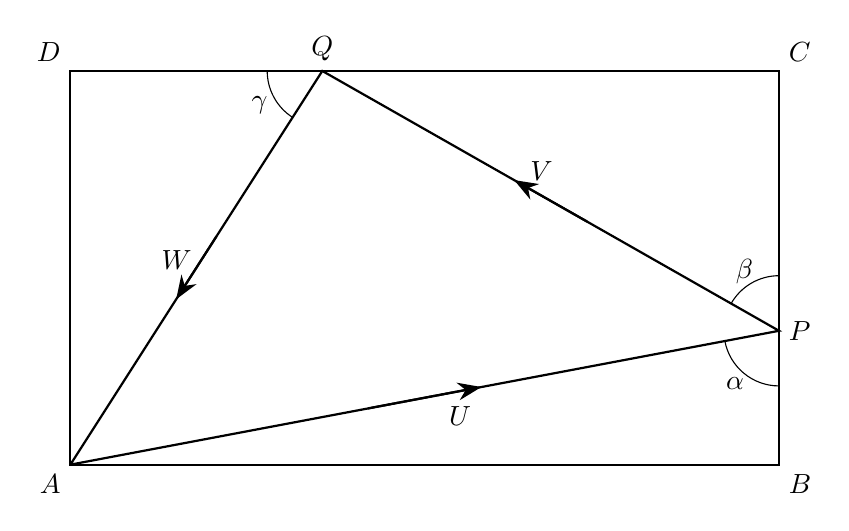
\begin{tikzpicture}[scale=1.0]
\def\W{9}
\def\H{5}
\def\Py{1.7}
\def\Qx{3.2}

\coordinate (A) at (0,0);
\coordinate (B) at (\W,0);
\coordinate (C) at (\W,\H);
\coordinate (D) at (0,\H);
\coordinate (P) at (\W,\Py);
\coordinate (Q) at (\Qx,\H);

\draw[thick] (A) -- (B) -- (C) -- (D) -- cycle;
\draw[thick] (A) -- (P) -- (Q) -- (A);

\draw[-{Stealth[length=3mm]}, thick] ($(A)!0.42!(P)$) -- ($(A)!0.58!(P)$);
\draw[-{Stealth[length=3mm]}, thick] ($(P)!0.42!(Q)$) -- ($(P)!0.58!(Q)$);
\draw[-{Stealth[length=3mm]}, thick] ($(Q)!0.42!(A)$) -- ($(Q)!0.58!(A)$);

\node[below, yshift=-2pt] at ($(A)!0.55!(P)$) {$U$};
\node[above, yshift=2pt] at ($(P)!0.52!(Q)$) {$V$};
\node[left] at ($(Q)!0.48!(A)$) {$W$};

\pic["$\alpha$", draw, angle radius=7mm, angle eccentricity=1.25] {angle=A--P--B};
\pic["$\beta$", draw, angle radius=7mm, angle eccentricity=1.25] {angle=C--P--Q};
\pic["$\gamma$", draw, angle radius=7mm, angle eccentricity=1.3] {angle=D--Q--A};

\node[below left] at (A) {$A$};
\node[below right] at (B) {$B$};
\node[above right] at (C) {$C$};
\node[above left] at (D) {$D$};
\node[right] at (P) {$P$};
\node[above] at (Q) {$Q$};
\end{tikzpicture}
\end{figure}


A small smooth billiard ball is projected from the corner $A$ of a horizontal rectangular table $ABCD$. \\

The ball first hits the side $BC$ at the point $P$, then hits the side $CD$ at the point $Q$, and then returns to $A$. \\

Angle $APB=\alpha$, angle $CPQ=\beta$ and angle $DQA=\gamma$. \\

The ball moves along $AP$ with speed $U$, along $PQ$ with speed $V$ and along $QA$ with speed $W$, as shown in the diagram. \\

The coefficient of restitution between the ball and side $BC$ is $e_1$. \\

The coefficient of restitution between the ball and side $CD$ is $e_2$. \\

The ball is modelled as a particle. \\

\begin{enumerate}[label=\textbf{(\alph*)}]
  \item Show that $\tan\beta=e_1\tan\alpha$. \marks{4} \\
  \item Hence show that $e_1\tan\alpha\tan\gamma=e_2$. \marks{3} \\
  \item By considering $\angle PAQ$ or otherwise, show that it is possible for the ball to return to $A$ only if $e_2>e_1$. \marks{6} \\
\end{enumerate}

If instead $e_1=e_2$, the ball would not return to $A$. \\

\begin{enumerate}[label=\textbf{(\alph*)}, resume]
  \item Given that $e_1=e_2$, use the result from part (b) to describe the path of the ball after it hits $CD$ at $Q$, explaining your answer. \marks{1} \\
\end{enumerate}
\newpage

% ---- Question 7 ----
\questionitem
% [Source: _QBT__Collisions_in_2_Dimensions, Q7]

A particle $P$ is moving with velocity $(7\mathbf{i}-4\mathbf{j})\,\mathrm{m\,s^{-1}}$ on a smooth horizontal plane. It collides with a smooth vertical wall which is parallel to the direction vector $2\mathbf{i}+\mathbf{j}$ and rebounds with velocity $(2\mathbf{i}+6\mathbf{j})\,\mathrm{m\,s^{-1}}$. \\

The coefficient of restitution between $P$ and this wall is $e$. \\

\begin{enumerate}[label=\textbf{(\alph*)}]
  \item Find the value of $e$. \marks{5} \\
\end{enumerate}
After this collision, $P$ goes on to hit a second smooth vertical wall which is parallel to the direction vector $\mathbf{i}-2\mathbf{j}$. The coefficient of restitution between $P$ and this second wall is $\dfrac{1}{2}$. \\

The angle through which the direction of motion of $P$ is deflected by its collision with this second wall is $\alpha^\circ$. \\

\begin{enumerate}[label=\textbf{(\alph*)}, resume]
  \item Find the value of $\alpha$, giving your answer to the nearest whole number. \marks{5} \\
\end{enumerate}

\newpage


% ---- Question 8 ----
\questionitem
% [Source: _QBT__Collisions_in_2_Dimensions, Q8]

\begin{figure}[H]
    \centering
\begin{tikzpicture}[scale=1.7]
\def\wallx{6}
\def\wallh{5.2}
\def\qy{2.8}
\def\px{4.6}
\def\rin{2.2}
\def\rout{2.2}

\coordinate (A) at (2,0);
\coordinate (B) at (\wallx,0);
\coordinate (C) at (\wallx,\wallh);
\coordinate (Q) at (\wallx,\qy);
\coordinate (P) at (\px,0);
\coordinate (R) at ($(Q)+(135:\rin)$);
\coordinate (S) at ($(P)+(120:\rout)$);

\draw[thick] (A) -- (B);
\draw[thick] (B) -- (C);

\draw[thick] (R) -- (Q) -- (P) -- (S);

\draw[-{Stealth[length=3mm]}, thick] ($(R)!0.38!(Q)$) -- ($(R)!0.56!(Q)$);
\draw[-{Stealth[length=3mm]}, thick] ($(Q)!0.38!(P)$) -- ($(Q)!0.58!(P)$);
\draw[-{Stealth[length=3mm]}, thick] ($(P)!0.36!(S)$) -- ($(P)!0.56!(S)$);

\pic["$45^\circ$", draw, angle radius=7mm, angle eccentricity=1.35] {angle=C--Q--R};
\pic["$60^\circ$", draw, angle radius=7mm, angle eccentricity=1.35] {angle=S--P--A};

\draw[thick] ($(B)+(-0.28,0)$) -- ++(0,0.28) -- ++(0.28,0);

\node[left] at (A) {$A$};
\node[right] at (B) {$B$};
\node[above right] at (C) {$C$};
\node[below] at (P) {$P$};
\node[right] at (Q) {$Q$};
\node[below left] at ($(R)!0.45!(Q)$) {$u$};
\end{tikzpicture}
\end{figure}


The diagram above represents the plan view of part of a horizontal floor, where $AB$ and $BC$ are perpendicular vertical walls.

The floor and the walls are modelled as smooth. \\

A ball is projected along the floor towards $BC$ with speed $u\,\mathrm{m\,s^{-1}}$ on a path at an angle of $45^\circ$ to $BC$. The ball hits $BC$ at $Q$ and then hits $AB$ at $P$. After striking $AB$, the ball moves away on a path at an angle of $60^\circ$ to $AB$. \\

The ball is modelled as a particle. \\

The coefficient of restitution between the ball and wall $BC$ is $\dfrac{1}{2}$. \\

\begin{enumerate}[label=\textbf{(\alph*)}]
  \item Find the coefficient of restitution between the ball and wall $AB$ and hence show that, using this model, the final kinetic energy of the ball is $50\%$ of the initial kinetic energy of the ball. \marks{8} \\
  \item In practice the walls and the floor may not be smooth. Explain how this model is likely to affect the percentage of kinetic energy remaining. \marks{1} \\
\end{enumerate}

\newpage

% ---- Question 9 ----
\questionitem
% [Source: _QBT__Collisions_in_2_Dimensions, Q9]

\begin{figure}[H]
    \centering
\begin{tikzpicture}[scale=1.5]
\def\wallleft{-1.5}
\def\wallright{6.5}
\def\uppery{3.8}
\def\px{0.8}
\def\qx{4.6}
\def\inlen{2.4}
\def\outlen{2.5}
\def\inang{140}
\def\outang{-25}
\coordinate (A) at (\wallleft,0);
\coordinate (B) at (\wallright,0);
\coordinate (C) at (\wallleft,\uppery);
\coordinate (D) at (\wallright,\uppery);
\coordinate (P) at (\px,0);
\coordinate (Q) at (\qx,\uppery);
\coordinate (S) at ($(P)+(\inang:\inlen)$);
\coordinate (R) at ($(Q)+(\outang:\outlen)$);

\draw[thick] (A) -- (B);
\draw[thick] (C) -- (D);
\draw[thick] (S) -- (P) -- (Q) -- (R);

\draw[-{Stealth[length=3mm]}, thick] ($(S)!0.28!(P)$) -- ($(S)!0.58!(P)$);
\draw[-{Stealth[length=3mm]}, thick] ($(P)!0.32!(Q)$) -- ($(P)!0.62!(Q)$);
\draw[-{Stealth[length=3mm]}, thick] ($(Q)!0.25!(R)$) -- ($(Q)!0.55!(R)$);

\pic["$\alpha$", draw, angle radius=8mm, angle eccentricity=1.35]{angle=S--P--A};
\pic[
  "$\tfrac{\pi}{4}-\alpha$"{yshift=2pt},
  draw,
  angle radius=10mm,
  angle eccentricity=1.65
]{angle=R--Q--D};

\node[below] at (A) {$A$};
\node[below] at (B) {$B$};
\node[above] at (C) {$C$};
\node[above] at (D) {$D$};
\node[left, yshift=-3pt] at ($(S)!0.48!(P)$) {$v\ \mathrm{m\,s^{-1}}$};
\end{tikzpicture}
\end{figure}


The diagram above represents the plan view of part of a horizontal floor, where $AB$ and $CD$ represent fixed vertical walls, with $AB$ parallel to $CD$. \\

A small ball is projected along the floor towards wall $AB$. Immediately before hitting wall $AB$, the ball is moving with speed $v\,\mathrm{m\,s^{-1}}$ at an angle $\alpha$ to $AB$, where $0<\alpha<\dfrac{\pi}{4}$. \\

The ball hits wall $AB$ and then hits wall $CD$. \\

Immediately after the impact with wall $CD$, the ball is moving at an angle $\dfrac{\pi}{4}-\alpha$ to $CD$. \\

The coefficient of restitution between the ball and wall $AB$ is $\dfrac{3}{5}$. \\

The coefficient of restitution between the ball and wall $CD$ is $\dfrac{1}{2}$. \\

The floor and the walls are modelled as being smooth. The ball is modelled as a particle. \\

\begin{enumerate}[label=\textbf{(\alph*)}]
  \item Show that
  \[
  \tan\alpha=\dfrac{2}{3}
  \] \marks[-20pt]{7}
  \item Find the percentage of the ball's initial kinetic energy that is lost in the two impacts. \marks{4} \\
\end{enumerate}


\newpage

% ---- Question 10 ----
\questionitem
% [Source: _QBT__Collisions_in_2_Dimensions, Q10]

A particle $P$ of mass $m$ is moving downwards and to the right in a direction making an angle $45^\circ$ with the horizontal when it strikes a fixed smooth inclined plane. The plane is inclined to the horizontal at an angle $\alpha$, where $0<\alpha<45^\circ$. \\

At the instant immediately before the impact, the speed of $P$ is $u$. \\

At the instant immediately after the impact, $P$ is moving upwards and to the right in a direction making an angle $45^\circ$ with the horizontal, with speed $v$. \\

\begin{enumerate}[label=\textbf{(\alph*)}]
  \item Show that the magnitude of the impulse exerted on the plane by $P$ is $mu \sec(45^\circ-\alpha)$. \marks{5} \\
\end{enumerate}
The coefficient of restitution between $P$ and the plane is $e$, where $0<e<1$. \\

\begin{enumerate}[label=\textbf{(\alph*)}, resume]
  \item Show that
  \[
  v^2=u^2\left(\cos^2(45^\circ+\alpha)+e^2\sin^2(45^\circ+\alpha)\right)
  \] \marks[-30pt]{3}
  \item Show that the kinetic energy lost by $P$ in the impact is
  \[
  \dfrac{1}{2} m u^2 (1-e^2)\sin^2(45^\circ+\alpha)
  \] \marks[-30pt]{2}
  \item Hence find, in terms of $m$, $u$ and $e$ only, the kinetic energy lost by $P$ in the impact. \marks{2} \\
\end{enumerate}

\newpage


% ---- Question 11 ----
\questionitem
% [Source: _QBT__Collisions_in_2_Dimensions, Q11]

\begin{figure}[H]
    \centering
\begin{tikzpicture}[scale=1.2]
\def\walllen{3.8}
\def\vinlen{3.5}
\def\voutlen{2.9}
\pgfmathsetmacro{\wallang}{atan2(4,3)}
\pgfmathsetmacro{\ain}{atan2(-7,26)}
\pgfmathsetmacro{\aout}{atan2(17,-6)}
\pgfmathsetmacro{\ainstart}{\ain+180}

\coordinate (P) at (0,0);
\coordinate (A) at ($(P)+(\wallang+180:\walllen)$);
\coordinate (B) at ($(P)+(\wallang:\walllen)$);
\coordinate (VinStart) at ($(P)+(\ainstart:\vinlen)$);
\coordinate (VoutEnd) at ($(P)+(\aout:\voutlen)$);

\draw[thick] (A) -- (B);
\draw[-{Stealth[length=3mm]}, thick] (VinStart) -- (P)
  node[midway, below left] {$(26\mathbf{i}-7\mathbf{j})\,\mathrm{m\,s}^{-1}$};
\draw[-{Stealth[length=3mm]}, thick] (P) -- (VoutEnd)
  node[pos=0.72, left] {$\mathbf{v}\,\mathrm{m\,s}^{-1}$};

\node[below left] at (A) {$A$};
\node[above right] at (B) {$B$};
\node[below right] at (P) {$P$};
\end{tikzpicture}
\end{figure}


The diagram above represents the plan view of part of a smooth horizontal billiards table, where $AB$ is a fixed smooth cushion. \\

The direction of $\overrightarrow{AB}$ is parallel to the vector $(3\mathbf{i}+4\mathbf{j})$. \\

A small disc of mass $0.2\,\mathrm{kg}$ is moving on the table when it strikes the cushion $AB$. \\

Immediately before impact with $AB$, the velocity of the disc is $(26\mathbf{i}-7\mathbf{j})\,\mathrm{m\,s^{-1}}$. \\

Immediately after impact with $AB$, the velocity of the disc is $\mathbf{v}\,\mathrm{m\,s^{-1}}$. \\

The coefficient of restitution between the disc and the cushion is $\dfrac{3}{5}$. \\

By modelling the disc as a particle, \\

\begin{enumerate}[label=\textbf{(\alph*)}]
  \item show that $\mathbf{v}=-6\mathbf{i}+17\mathbf{j}$ \marks{6} \\
  \item Find the magnitude of the impulse exerted by the cushion on the disc in the impact. \marks{3} \\
\end{enumerate}

\newpage


% ---- Question 12 ----
\questionitem
% [Source: _QBT__Collisions_in_2_Dimensions, Q12]

\begin{figure}[H]
    \centering
\begin{tikzpicture}[scale=1.2]
\def\xB{5}
\def\yC{4.6}
\def\xP{3.5}
\def\yQ{3}
\def\xD{3.5}
\def\yD{5}
\def\xE{1.5}
\def\yE{3}
\def\ra{0.22}

\coordinate (A) at (0,0);
\coordinate (B) at (\xB,0);
\coordinate (C) at (\xB,\yC);
\coordinate (P) at (\xP,0);
\coordinate (Q) at (\xB,\yQ);
\coordinate (D) at (\xD,\yD);
\coordinate (E) at (\xE,\yE);

\draw[thick] (A) -- (B);
\draw[thick] (B) -- (C);

\draw[thick] (D) -- (Q);
\draw[-{Stealth[length=3mm]}, thick] ($(D)!0.35!(Q)$) -- ($(D)!0.55!(Q)$);
\draw[thick] (Q) -- (P);
\draw[-{Stealth[length=3mm]}, thick] ($(Q)!0.3!(P)$) -- ($(Q)!0.55!(P)$);
\draw[thick] (P) -- (E);
\draw[-{Stealth[length=3mm]}, thick] ($(P)!0.25!(E)$) -- ($(P)!0.45!(E)$);

\pic["$\alpha$", draw, angle radius=6mm, angle eccentricity=1.4] {angle=C--Q--D};
\pic["$\beta$", draw, angle radius=9mm, angle eccentricity=1.4] {angle=P--Q--B};

\draw[thick] ($(B)+(-\ra,0)$) -- ($(B)+(-\ra,\ra)$) -- ($(B)+(0,\ra)$);

\node[below left] at (A) {$A$};
\node[below right] at (B) {$B$};
\node[above right] at (C) {$C$};
\node[below left] at ($(D)!0.5!(Q)$) {$10\,\mathrm{m\,s}^{-1}$};
\end{tikzpicture}
\end{figure}


The diagram above represents the plan view of one corner of a smooth air-hockey table, where $AB$ and $BC$ are fixed cushions with $AB$ perpendicular to $BC$. \\

A small puck is struck along the table towards $BC$ with speed $10\,\mathrm{m\,s^{-1}}$ on a path that makes an angle $\alpha$ with $BC$, where $\tan \alpha = \dfrac{3}{4}$. The puck hits $BC$ and then hits $AB$. \\

Immediately after hitting $BC$, the puck is moving at an angle $\beta$ to $BC$, where $\tan \beta = \dfrac{1}{2}$. \\

The coefficient of restitution between the puck and $BC$ is $e$. \\

The coefficient of restitution between the puck and $AB$ is $\dfrac{3}{4}$. \\

By modelling the puck as a particle and the table and cushions as being smooth, \\

\begin{enumerate}[label=\textbf{(\alph*)}]
  \item show that $e = \dfrac{2}{3}$ \marks{5} \\
  \item find the speed of the puck immediately after it hits $AB$. \marks{4} \\
  \item Suggest two ways in which the model could be refined to make it more realistic. \marks{2} \\
\end{enumerate}
\end{enumerate}
\end{document}
